% !TEX root = ../intro-stellar-physics.tex

\newcommand*{\DDtt}[1]{\frac{\dif^{2} #1}{\dif t^{2}}}
\newcommand*{\wt}{\omega t}
\newcommand*{\wot}{\omega_{0} t}
\newcommand*{\wmt}{\omega_{m} t}
\newcommand*{\womw}{(\omega_{0}^{2}-\omega^{2})}
\newcommand*{\gw}{\Gamma^{2}\omega^{2}}

\nocite{Mihalas1978Stellar-Atmosph,LeBlanc2010An-Introduction,Carroll2006An-Introduction}

\section{Warmup: the simple harmonic oscillator}

Let's begin with a simple system: a mass $m$ attached to a spring with force constant $k$. 

\subsection{With no driving force}

\begin{marginfigure}
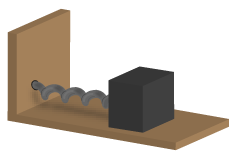
\includegraphics[width=\linewidth]{simple-spring}
\caption[A simple harmonic oscillator]{A simple harmonic oscillator: a mass $m$ on a frictionless surface attached to a  spring with force $F = -kx$.
\label{f.simple-spring}}
\end{marginfigure}

If we put the origin of our coordinate system where the mass is at rest with the spring relaxed, then the equation of motion of the mass is
\begin{equation}\label{e.SHO-basic}
	\DDtt{x} + \frac{k}{m} x = 0.
\end{equation}
You have solved this before: the most general solution is
\begin{equation}\label{e.SHO-general-solution}
	x(t) = x_{0}\cos(\wot) + \frac{v_{0}}{\omega_{0}}\sin(\wot)
\end{equation}
with $\omega_{0}^{2} = k/m$ and with $x_{0}$ and $v_{0}$ being the initial position and velocity of the mass.

\subsection{With driving at frequency $\omega \neq \omega_{0}$}

Now let's push on our mass with an oscillating force, $F\cos(\omega t)$ with $\omega\neq\omega_{0}$. A real world example would be holding a vibrating tuning fork near another fork tuned to a different frequency.  The equation of motion is now
\begin{equation}\label{e.SHO-driven}
	\DDtt{x} + \omega_{0}^{2}x = \frac{F}{m}\cos(\wt).
\end{equation}
You can verify by substitution that a general solution is
\[
	x(t) = \frac{F/m}{(\omega_{0}^{2}-\omega^{2})}\cos(\wt) + A\cos(\wot)+B\sin(\wot).
\]
Let's start with our harmonic oscillator at rest ($v_{0} = \left.\dif x/\dif t\right|_{t=0} = 0$) and at $\left. x\right|_{t=0} = 0$.  With these conditions, we can determine the constants $A$ and $B$; the solution is
\[
	x(t) = \frac{F/m}{(\omega_{0}^{2}-\omega^{2})}\left[\cos(\wt)-\cos(\wot)\right].
\]
Let's recast this by defining $\Delta = \omega_{0} - \omega$ and $\omega_{m} = (\omega_{0}+\omega)/2$.  Then
\begin{eqnarray*}
  \omega_{0}^{2}-\omega^{2} &=& (\omega_{0}-\omega)(\omega_{0}+\omega) = 2\Delta\omega_{m},\\
  \cos(\wot) &=& \cos\left(\wmt+\Delta t/2\right) = \cos(\wmt)\cos(\Delta t/2) - \sin(\wmt)\sin(\Delta t/2),\\
  \cos(\wt) &=& \cos\left(\wmt-\Delta t/2\right) = \cos(\wmt)\cos(\Delta t/2) + \sin(\wmt)\sin(\Delta t/2);
\end{eqnarray*}
and we write the solution as
\begin{equation}\label{e.beats}
	x(t) = \left[\frac{F/m}{\Delta\omega_{m}}\sin(\Delta t/2)\right]\sin(\wmt).
\end{equation}
This illustrates the phenomena of \textbf{beats}: the oscillation consists of a carrier signal at frequency $\omega_{m}$ with the amplitude modulated at the slower frequency $\Delta /2$.  Notice that the amplitude increases as $\Delta \to0$, i.e., $\omega\to\omega_{0}$.

\subsection{With both driving and damping}

Now let's make our model even more realistic by adding some \textbf{damping}.  We add a frictional force that is proportional to velocity, $F_{\mathrm{friction}} = -m\Gamma \dif x/\dif t$. Our complete equation of motion is then
\begin{equation}
	\DDtt{x} + \Gamma \DDt{x} + \omega_{0}^{2}x = \frac{F}{m}\cos(\omega t).
\end{equation}
The solution to this is straightforward to find, although the algebra is tedious (trust me on this). The general solution for initial conditions $\left.x\right|_{t=0} = x_{0}$ and $\left.\dif x/\dif t\right|_{t=0} = v_{0}$ is
\begin{eqnarray}
\label{e.general-solution-ddo}
\lefteqn{x(t) = \frac{F\womw/m}{\womw^{2}+\gw}\cos(\omega t)} && \\
	&+& \frac{\Gamma\omega F/m}{\womw^{2}+\gw}\sin(\omega t)\nonumber \\
	&+& \left[x_{0}-\frac{F\womw/m}{\womw^{2}+\gw}\right]{\color{red}e^{-\Gamma t/2}} \cos(\omega_{\Gamma}t) \nonumber\\
	&+& \left[\frac{v_{0}}{\omega_{\Gamma}}-\frac{\Gamma\omega F/m}{\womw^{2}+\gw}
	\,\frac{\omega}{\omega_{\Gamma}}\right]{\color{red}e^{-\Gamma t/2}} \sin(\omega_{\Gamma}t), 
	\nonumber
\end{eqnarray}
with
\[ 
    \omega_{\Gamma} = 
        \omega_{0}\left(1-\frac{\Gamma^{2}}{4\omega_{0}^{2}}\right)^{1/2}.
\]
Let's simplify this to the most relevant case.  First, the last two terms decay as {\color{red}$e^{-\Gamma t/2}$}: these are transients set by the initial conditions. After a time $2/\Gamma$ there will only be the first two terms, which oscillate at frequency $\omega$. 

We can simplify these first two terms even further: write
\[ \cos(\wt) = \frac{e^{i\wt}+e^{-i\wt}}{2},\quad \sin(\wt) 
    = \frac{e^{i\wt}-e^{-i\wt}}{2i}; \]
and combine terms to find
\begin{eqnarray}
    x(t) &=& \frac{F}{2m}\left[\frac{1}{\left(\omega_0^2-\omega^2\right) + i\Gamma\omega}\right]e^{i\wt} + \frac{F}{2m}\left[\frac{1}{\left(\omega_0^2-\omega^2\right) - i\Gamma\omega}\right]e^{-i\wt} \nonumber\\
    &=& \Re\left\{\frac{F}{m}\left[\frac{1}{\left(\omega_0^2-\omega^2\right) + i\Gamma\omega}\right]e^{i\wt}\right\}\label{e.oscillator-expression}
\end{eqnarray}
We use the symbol ``$\Re$'' to denote taking the real part of a complex quantity.  

From Eq.~(\ref{e.oscillator-expression}), we see that the oscillator can be described as the real part of a complex quantity $Ae^{i\wt}$, with
\[
    A = \frac{F}{m}\left[\frac{1}{\left(\omega_0^2-\omega^2\right) + i\Gamma\omega}\right].
\]
For $\omega \approx \omega_0$, we write $(\omega_0^2-\omega^2)\approx 2\omega_0(\omega_0-\omega)$ and take the square of the amplitude to find,
\begin{eqnarray}
    \left|A\right|^2 &=& \left(\frac{F}{2m\omega_0}\right)^2
        \frac{1}{(\omega_0-\omega)^2 + (\Gamma/2)^2}\nonumber\\
    &=& \frac{\pi}{2\Gamma}\left(\frac{F}{m\omega_0}\right)^2
        \left\{\frac{1}{\pi}\frac{\Gamma/2}{(\omega_0-\omega)^2 + (\Gamma/2)^2}\right\}
\end{eqnarray}
We rewrote the amplitude in the second line so that the term in $\{\cdot\}$ is normalized. The function
\[
    \mathcal{L}(\omega;\Gamma) = \frac{1}{\pi} 
        \frac{\Gamma/2}{(\omega_0-\omega)^2 + (\Gamma/2)^2}
\]
is known as a Lorentzian.  In contrast to a Gaussian, a Lorentzian is characterized by broad ``wings'' (Fig.~\ref{f.comparison}) as it goes to zero away from the central frequency $\omega_{0}$.
\begin{marginfigure}[-4\baselineskip]
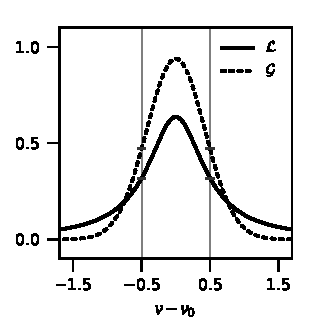
\includegraphics[width=\linewidth]{comparison}
\caption[Comparison of Lorentzian and Gaussian distributions]{\label{f.comparison}
Comparison of a Lorentzian ($\mathcal{L}$, solid line) and a Gaussian ($\mathcal{G}$, dotted line), both with $\mathrm{FWHM}=1$. The area under each curve is unity.}
\end{marginfigure}

\section{Atomic Lines}
You may be thinking, ``What does this have to do with atomic lines?'' Consider an electronic transition in an atom between two energy levels, $E_m$ and $E_n$. The natural frequency of this transition is $\nu_0 = |E_n-E_m|/h$. Light incident on the atom with frequency\sidenote{We are switching from angular frequency $\omega$ to frequency $\nu = \omega/2\pi$.} $\nu\neq\nu_0$ drives the electron at frequency $\nu$. An accelerating electron radiates, which damps the acceleration of the electron.  Classically, the transition in an atom is an electromagnetic oscillator with damping and driving terms, with cross-section\sidenote{For details, see the appendix.}
\begin{equation}\label{e.semi-classical}
    \sigma = \left(\frac{\pi e^2}{m_e c}\right)
    \left\{\frac{\Gamma/4\pi}{(\nu_0-\nu)^2 + (\Gamma/4\pi)^2}\right\}.
\end{equation}
The actual value of the cross-section must be calculated using quantum mechanics. The overall shape of the cross-section is still in the form of equation~(\ref{e.semi-classical}) with opacity
\begin{equation}
    \rho\kappa_\nu = n_i \left(\frac{\pi e^2}{m_e c}\right) f_{mn}
        \left\{\frac{\Gamma/4\pi}{(\nu_0-\nu)^2 + (\Gamma/4\pi)^2}\right\}.
\end{equation}
In this equation, $f_{mn}$ is a number, called the \emph{oscillator strength}, that results from the calculation of the transition probability from state $m$ to state $n$, and $n_i$ is the density of atoms in state $m$.  The key point is that $f_{mn}$ depends only on the details of the transition: the energies, spins, and parities of the atomic states.  It does not depend on environmental parameters such as temperature and pressure.  As a result, $f_{mn}$ can be measured or computed once and then tabulated.

There is an intrinsic width $\Gamma$ that is set by the finite lifetime of the energy levels; in practice, however, this is not important.  In a stellar atmosphere, the width $\Gamma$ is set by collisions.  For example, when an electron passes close by our atom, the electric field shifts the energy levels of the atom\sidenote{This is an application of the \emph{Stark} effect that you learn about in quantum mechanics.}.  The greater the collision rate, the larger the width.
If we have two stars of the same photospheric temperature (so that both stars have the same lines), then a way to increase the collision rate is to increase the pressure. Recall, however, that in the stellar atmosphere $P = (g/\kappa)\tau$; as a result, stars with a higher surface gravity will have broader lines. The inset in Figure~\ref{f.compare_grav} illustrates the broadening of the Balmer H$\gamma$ line ($5\to 2$) in the spectrum of a main-sequence A1 star compared with that of a supergiant A1 star.

\begin{figure}[hp]
    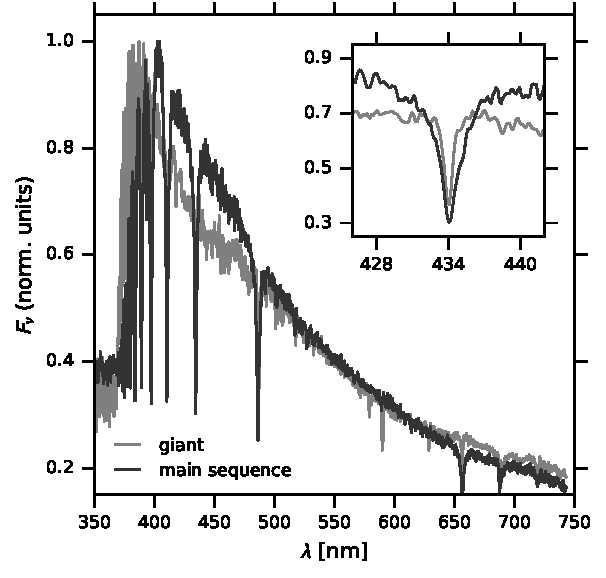
\includegraphics[width=\linewidth]{compare_grav}
    \caption[Spectra of two A1 stars]{\label{f.compare_grav}
    Spectra of two A1 stars, HD 16608 (a main sequence star) and SAO 12149 (a supergiant star).  Spectra are from \citet{Jacoby1984A-library-of-st}.
    }
\end{figure}

In addition to the width set by collisions, the line is also broadened by thermal motion: the atoms are in ceaseless motion; those headed towards us absorb at a blueshifted frequency, while those headed away from us absorb at a redshifted frequency.  Because the atomic velocities follow a Maxwell-Boltzmann distribution, the net effect is to make the core of the line (that is, near the center) assume a Gaussian profile.  Because a Gaussian falls off more quickly than a Lorentzian profile (see Fig.~\ref{f.comparison}), the wings of the line are still determined by the collision rate.

\section{A more detailed look}

This section is modified from Chapter 8 of \emph{Stellar Astrophyiscs}, \href{https://github.com/Open-Astrophysics-Bookshelf/stellar-physics-notes}{available} from The Open Astrophysics Bookshelf on GitHub.  In this section, Gaussian CGS units are used for the electromagnetic field. To convert to MKS, make the following substitutions:
\begin{eqnarray*}
e &\to& \frac{1}{\sqrt{4\pi\varepsilon_0}}e\\
\bvec{E} &\to& \sqrt{4\pi\varepsilon_0}\bvec{E}\\
c &\to& (\mu_0\varepsilon_0)^{-1/2}.
\end{eqnarray*}

\newthought{Suppose we have a classical charged harmonic oscillator.}  The instantaneous power emitted by the oscillator is
\begin{equation}\label{e.larmor-power}
	 P(t) = \frac{2}{3}\frac{e^{2}}{c^{3}} |\dot{\vu}|^{2},
\end{equation}
and when averaged over a cycle is
\begin{equation}\label{e.oscillator-power}
	 \left\langle P(t) \right\rangle = \frac{e^{2}}{3c^{3}}x_{0}^{2} \omega^{4},
\end{equation}
since $\dot{\vu} = -\omega^{2}\bvec{x}_{0}\cos \omega t$. Since the oscillator is radiating, it is losing energy and is damped. Let us write the damping as $\bvec{F}_{\mathrm{rad}}\vdot \vu$; to find $\bvec{F}_{\mathrm{rad}}$, we integrate the power loss over a cycle,
\[  -\int_{t_{1}}^{t_{2}}\!\dif t\;\frac{2}{3}\frac{e^{2}}{c^{3}}\dot{\vu}\vdot\dot{\vu} 
	= -\left.\frac{2}{3}\frac{e^{2}}{c^{3}}\dot{\vu}\vdot\vu\right|_{t_{1}}^{t_{2}} 
	+ \frac{2}{3}\frac{e^{2}}{c^{3}} \int_{t_{1}}^{t_{2}}\!\dif t\;\ddot{\vu}\vdot\vu. 
\]
Since the motion is periodic, the first term vanishes and we can therefore identify 
\[ 
	\bvec{F}_{\mathrm{rad}} = \frac{2}{3}\frac{e^{2}}{c^{3}}\ddot{\vu} 
	= -m\left(\frac{2e^{2}\omega^{2}}{3c^{3}m}\right)\vu
\]
as the radiation damping term with the term in parenthesis being the damping constant $\gamma$. 
If there is an driving electric field on our oscillator, then its equation of motion becomes
\begin{equation}\label{e.eq-sho}
	m\ddot{\bvec{x}} = -m\omega_{0}^{2}\bvec{x} + e\bvec{E}e^{i\omega t} - m\gamma \dot{\bvec{x}}.
\end{equation}
Using a trial function $\bvec{x}\propto e^{i\omega t}$ gives
\[
	\bvec{x} = \frac{e}{m}\frac{E e^{i\omega t}}{(\omega_{0}^{2}-\omega^{2}) + i\omega\gamma}.
\]
Taking the second derivative w.r.t.\ time of $\bvec{x}$, substituting into eq.~(\ref{e.larmor-power}), and averaging over a cycle gives the power radiated by the oscillator,
\[
	\left\langle P(t)\right\rangle = \frac{e^{4}\omega^{4} E^{2}}{3 c^{2}m^{2}}
	\frac{1}{(\omega_{0}^{2}-\omega^{2})^{2} + \gamma^{2}\omega^{2}}.
\]
Dividing $\langle P(t)\rangle$ by the incident power per unit area, $cE^{2}/(8\pi)$, gives the cross-section:
\begin{equation}\label{e.classical-oscillator-cross-section}
	\sigma = \frac{8\pi}{3}\frac{e^{4}}{m^{2}c^{3}}
	\frac{\omega^{4}}{(\omega_{0}^{2}-\omega^{2})^{2} + \gamma^{2}\omega^{2}}.
\end{equation}
Now, for $\omega \approx \omega_{0}$, we can expand $(\omega_{0}^{2}-\omega^{2})^{2} \approx 4\omega_{0}^{2}(\omega_{0}-\omega)^{2}$; furthermore, we identify $2e^{2}\omega_{0}^{2}/(3c^{3}m) = \gamma$ and equation~(\ref{e.classical-oscillator-cross-section}) becomes
\begin{equation}\label{e.cross-section-lorentz}
	\sigma = \pi\left(\frac{e^{2}}{mc}\right)\frac{\gamma}{(\omega_{0}-\omega)^{2} + (\gamma/2)^{2}}.
\end{equation}
The line profile is Lorentzian, with a width $\gamma$. In terms of wavelength, the width is
\[ 
	\Delta \lambda = \left|\frac{\dif\lambda}{\dif\omega}\right|\gamma = \frac{2\pi c}{\omega^{2}}\gamma
	= \val{\sci{1.2}{-4}}{\textrm{\AA}}.
\]
This width is independent of the transition frequency (it is just the classical electron radius), and it is very, very small.  In a stellar atmosphere, the width is set by interactions and doppler broadening.

\newthought{To understand how impacts affect the line width}, suppose we model the oscillator as being started and stopped by impacts; in between impacts it just goes as $e^{i\omega_{0}t}$.  To get the spectrum, we take the Fourier transform,
\[
	F(\omega,t) = \int_{0}^{t}\!\dif t'\; \exp[i(\omega_{0}-\omega)t'],
\]
where $t$ is some time between impacts. Now if the impacts are distributed randomly and are uncorrelated, then the distribution of wait times follows a Poisson distribution,
\[ W(t)\,\dif t = e^{-t/\tau}\,\dif t/\tau, \]
where $\tau$ is the average time between collisions.  Using this to compute the energy spectrum, we obtain
\[ E(\omega) = \frac{1}{2\pi\tau}\int_{0}^{\infty}\!\dif t\; F(\omega,t)F^{*}(\omega,t)W(t) = \frac{1}{\pi\tau} 
	\frac{1}{(\omega_{0}-\omega)^{2} + (1/\tau)^{2}};
\]
the line profile is again Lorentzian, with a FWHM $2/\tau$.

We might be inclined to treat the atoms as hard spheres, but this gives a large $\tau$, or equivalently a narrow line width. We are therefore led to consider longer-range interactions for setting the intrinsic line width. Table~\ref{t.perturbers} lists such interactions. For a given impact parameter, the interaction perturbs the energy levels; by integrating over a distribution of  impact parameters one gets the intrinsic damping. Of course, we should really use a quantum mechanical calculation.  We can scale our cross-section to the classical result (eq.~[\ref{e.cross-section-lorentz}]), however, by writing
\begin{equation}\label{e.cross-section}
	 \sigma_{\nu} = \left(\frac{\pi e^{2}}{m_{e}c}\right) f \phi_{\nu}, 
\end{equation}
where $\phi_{\nu}$ is the line profile (dimension $\sim \Hz^{-1}$) and $f$ is a dimensionless cross-section called the \textbf{oscillator strength}.

\begin{table}[htbp]
\caption{Interactions in stellar atmospheres}\label{t.perturbers}
\begin{tabular}{crcc}
\hline
perturbation & form & source & affects\\
\hline\hline
linear Stark & $C_{2} r^{-2}$ & $e^{-}$, $p$, ions & H (H$\alpha$, H$\beta$, \ldots)\\
quadratic Stark & $C_{4} r^{-4}$ & $e^{-}$ & non-hydrogenic ions\\
van der Waals & $C_{6}r^{-6}$ & atoms, H & most atomic lines, esp.\ in cool stars\\
\hline
\end{tabular}
\end{table}
